\documentclass[12pt]{article}
\usepackage{polski}
\usepackage[utf8]{inputenc}
\usepackage{amsfonts}
\usepackage{amsmath}
\usepackage{enumitem}
\usepackage{graphicx}
\usepackage{float}
\usepackage{centernot}
\setlength{\parskip}{1em}


\begin{document}
	\title{Sprawozdanie\\Metody Numeryczne 2, laboratorium 4}
	\author{Grzegorz Rozdzialik (D4, grupa lab. 2)}
	\maketitle	
	
	\section{Zadanie}
	{\Large Temat \textbf{4}, zadanie \textbf{46}:}\\
	Wzory empiryczne. Baza: $1$, $x$, $x^2$, $\sin x$. Graficzne przedstawienie punktów pomiarowych i funkcji przybliżającej.
	
	Niech $f: \mathbb{R} \to \mathbb{R}$ będzie funkcją aproksymowaną,
	$m \in \mathbb{R}$,
	$x_1, x_2, \dots, x_m \in \mathbb{R}$
	oraz $f_1, f_2, \dots, f_m \in \mathbb{R}$ będą wartościami funkcji aproksymowanej w punktach $x_i$ ($f_i = f(x_i), i = 1, 2, \dots, m$).
	
	Niech $g_1, g_2, \dots, g_n: \mathbb{R} \to \mathbb{R}$ będą funkcjami z bazy.
	
	Należy znaleźć element optymalny
	\begin{equation}
	f^* = \alpha_1 g_1(x) + \alpha_2 g_2(x) + \dots + \alpha_n g_n(x) \label{element-optymalny}
	\end{equation},
	który minimalizuje wyrażenie
	\begin{equation}
	H(\alpha_1, \alpha_2, \dots, \alpha_n) = \sum_{i=1}^{m} \Big(f_i - f^*(x_i)\Big)^2
	\label{funkcja-H}
	\end{equation}
	Zakładamy $m \geq n$.
	
	
	\section{Opis metody}
	Po obliczeniu pochodnej funkcji $H$ (równanie \eqref{funkcja-H}) ze względu na dowolną zmienną $\alpha_i$ i przyrównaniu jej do zera (ponieważ szukamy ekstremum) otrzymujemy następującą równość:
	\begin{equation}
		\forall_{k = 1, \dots, n} \hspace{10pt}
		\sum_{j=1}^{n} \alpha_j \sum_{i=1}^{m} g_j(x_i) g_k(x_i) = \sum_{i=1}^{m} f_i g_k(x_i)
		\label{rownosc-pochodnej-trudna}
	\end{equation}
	Zauważmy, że $\sum_{i=1}^{m} g_j(x_i) g_k(x_i) = \langle g_j, g_k \rangle$ oraz 
	$\sum_{i=1}^{m} f_i g_k(x_i) = \langle f_i, g_k \rangle$. Zatem równość \eqref{rownosc-pochodnej-trudna} można zapisać jako:
	\begin{equation}
		\forall_{k = 1, \dots, n} \hspace{10pt}
		\sum_{j=1}^{n} \alpha_j \langle g_j, g_k \rangle = \langle f_i, g_k \rangle
		\label{rownosc-pochodnej-uproszczona}
	\end{equation}
	
	Otrzymaliśmy więc układ równań normalnych $G \alpha = F$, gdzie
	\begin{equation*}
		\alpha =
		\begin{bmatrix}
			\alpha_1 \\
			\alpha_2 \\
			\vdots   \\
			\alpha_n
		\end{bmatrix}
	\end{equation*}
	\begin{equation*}
		G =
		\begin{bmatrix}
			\langle g_1, g_1 \rangle & \langle g_1, g_2 \rangle & \dots  & \langle g_1, g_n \rangle \\
			\langle g_2, g_1 \rangle & \langle g_2, g_2 \rangle & \dots  & \langle g_2, g_n \rangle \\
			\vdots                   & \vdots                   & \ddots & \vdots                   \\
			\langle g_n, g_1 \rangle & \langle g_n, g_2 \rangle & \dots  & \langle g_n, g_n \rangle
		\end{bmatrix}
	\end{equation*}
	\begin{equation*}
		F =
		\begin{bmatrix}
			\langle f_1, g_1 \rangle \\
			\langle f_2, g_2 \rangle \\
			\vdots                   \\
			\langle f_n, g_n \rangle
		\end{bmatrix}
	\end{equation*}
	Po jego rozwiązaniu otrzymujemy współczynniki $\alpha_i$, a mamy całą postać elementu optymalnego $f^*$.



	W przypadku naszego zadania mamy:
	\begin{align*}
	g_1(x) &= 1\\
	g_2(x) &= x\\
	g_3(x) &= x^2\\
	g_4(x) &= \sin x
	\end{align*}
	Ilość punktów pomiarowych $n$ nie może być mniejsza niż 4 ($n \geq 4$). Wtedy element optymalny $f^*$ ma postać:
	$$
	f^*(x) = \alpha_1 + \alpha_2 x + \alpha_3 x^2 + \alpha_4 \sin x
	$$
	
	Po obliczeniu iloczynów skalarnych $\langle g_i, g_j \rangle$ (dla $i, j = 1, 2, 3, 4$) i wstawieniu do macierzy $G$ otrzymujemy:
	\begin{align*}
		G = \sum_{k=1}^{m}
		\begin{bmatrix}
			m        & x_k          & x_k^2          & \sin x_k     \\
			x_k      & x_k^2        & x_k^3          & x_k \sin x_k \\
			x_k^2    & x_k^3        & x_k^5 x_k^2    & \sin x_k     \\
			\sin x_k & x_k \sin x_k & x_k^2 \sin x_k & \sin^2 x_k
		\end{bmatrix}
	\end{align*}
	
	 Po obliczeniu iloczynów skalarnych $\langle f_i, g_i \rangle$ (dla $i = 1, 2, 3, 4$) i wstawieniu do wektora $F$ otrzymujemy:
	 \begin{align*}
		 F = \sum_{k=1}^{m}
		 \begin{bmatrix}
		 	f_k          \\
		 	f_k x_k      \\
		 	f_k x_k^2    \\
		 	f_k \sin x_k
		 \end{bmatrix}
	 \end{align*}
	 
	 Zatem należy rozwiązać układ równań $G\alpha = F$, gdzie
	 $$
 	\alpha = 
 	\begin{bmatrix}
 		\alpha_1 \\
 		\alpha_2 \\
 		\alpha_3 \\
 		\alpha_4
 	\end{bmatrix}
	 $$
	 
	Element optymalny $f^*$ otrzymujemy wstawiając znalezione współczynniki $\alpha_1, \dots, \alpha_4$ do wzoru \eqref{element-optymalny}.
	
	
	
	\section{Implementacja metody}
	Implementacja metody podzielona jest na następujące kroki:
	\begin{enumerate}
		\item Obliczenie macierzy $G$ oraz wektora $F$ na podstawie podanych punktów pomiarowych (funkcja \texttt{computeApproximationEquation}).
		\item Obliczenie współczynników $\alpha_1, \dots, \alpha_4$ (funkcja \texttt{computeApproximationCoefficients}).
		\item Uzyskanie elementu optymalnego (funkcja \texttt{composeApproximationFunction}).
	\end{enumerate}

	
	
	\section{Poprawność metody}
	Dla przykładowych punktów pomiarowych testowanych przeze mnie metoda była poprawna, to jest znajdowała funkcję, która aproksymowała te punkty. Zdarzało się jednak, że aproksymacja ta nie była zbyt dokładna.
	
	Zatem ogólnie można stwierdzić, że metoda jest poprawna. W swoich obliczeniach w sekcji 2 nie stosowałem żadnych restrykcyjnych założeń, zatem powinna być wykonalna dla wszystkich zestawów punktów pomiarowych, z zastrzeżeniem, że dla niektórych może nie być dokładna.
	
	
	
	
	\section{Przykłady}
	\textbf{TODO}
	
	\begin{enumerate}[label=\textbf{Przykład \arabic*}]
		\item
		\textbf{TODO}
		
	\end{enumerate}
	
	
	
	
	
	
	\section{Wnioski}
	\begin{enumerate}
		\item Element optymalny w tym przypadku odwzorowuje dokładnie funkcje z bazy.
		\item Dla 4 punktów pomiarowych aproksymacja jest dokładna (staje się interpolacją). Dla większej ilości punktów nie ma takiej zależności.
		\item Im więcej punktów pomiarowych i im większe moduły zmian między nimi, tym aproksymacja jest gorsza.
	\end{enumerate}
	
	
	
	\section{Funkcja do testowania metody}
	Funkcja \texttt{plotApproximation(x, f, pointsCount, paddingMultiplier)} umożliwia łatwe testowanie metody. Oblicza ona element optymalny, a następnie wyświetla wykres elementu optymalnego oraz nanosi na niego punkty pomiarowe.
	
	Obszar, na jakim rysowany jest wykres jest powiększony o $paddingMultiplier * (\max_{i \in {1, \dots, m}} x_i - \min_{i \in {1, \dots, m}} x_i)$ w celu zobrazowania elementu optymalnego również poza zakresem punktów pomiarowych. Domyślna wartość $paddingMultiplier = \frac{1}{6}$.
	
	Argumenty przyjmowane przez tą funkcję opisane są w pliku \textit{plotApproximation.m} (nad nagłówkiem funkcji).
	
	Przykładowe wywołanie funkcji:
	\texttt{plotApproximation([0 1 2 3], [5 6 8 -5])}
	
	
	\section{Interfejs graficzny}
	Do metody został dołączony interfejs graficzny umożliwiający łatwe wprowadzanie punktów pomiarowych, zmianę parametrów (współczynnik powiększenia obszaru, a także ilość punktów wewnątrz obszaru, na których zostanie narysowany wykres) i dokonanie z tymi danymi aproksymacji.
	
	\begin{figure}[H]
		\centering
		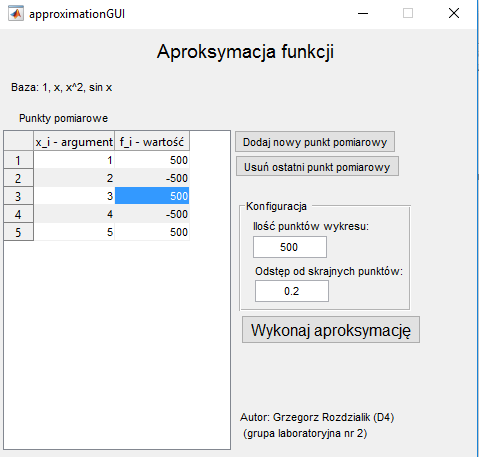
\includegraphics[scale=1]{images/gui.png}
		\caption{Interfejs graficzny}
		\label{GUI}
	\end{figure}
	
	
	
	\section{Bibliografia}
	\begin{enumerate}
		\item Informacje z wykładu \textit{Metod numerycznych 2} (wydział MiNI PW, dr Iwona Wróbel) \textbf{TODO} (dodać więcej informacji)
	\end{enumerate}
	
\end{document}